\documentclass[10pt]{article}

% Redo, replot, rewrite.
\usepackage{research}
\usepackage{setspace}
\usepackage{float}
\usepackage{subcaption}
\usepackage{listings}
\usepackage[small]{titlesec}
\usepackage[T1]{fontenc}
\usepackage{bigfoot} % to allow verbatim in footnote
\usepackage[numbered,framed]{matlab-prettifier}
\lstset{
	style              = Matlab-editor,
	basicstyle         = \mlttfamily,
	escapechar         = ",
	mlshowsectionrules = true,
}
\setlength{\baselineskip}{20pt}
\DeclareMathOperator{\x}{\mathbf{x}}
\DeclareMathOperator{\uo}{\mathbf{u_0}}
\DeclareMathOperator{\bu}{\mathbf{u}}
\DeclareMathOperator{\Hs}{\mathcal{H}}

\title{\textbf{\large{ECE 271A Problem Set 5.}}}

\author{Jun Hao (Simon) Hu}
\date{\today}

\begin{document}

\maketitle

\section{Part 1, $C = 8$.}
\subsection{Results.}
\begin{figure}[H]
	\begin{subfigure}{0.5\textwidth}
		\centering 
		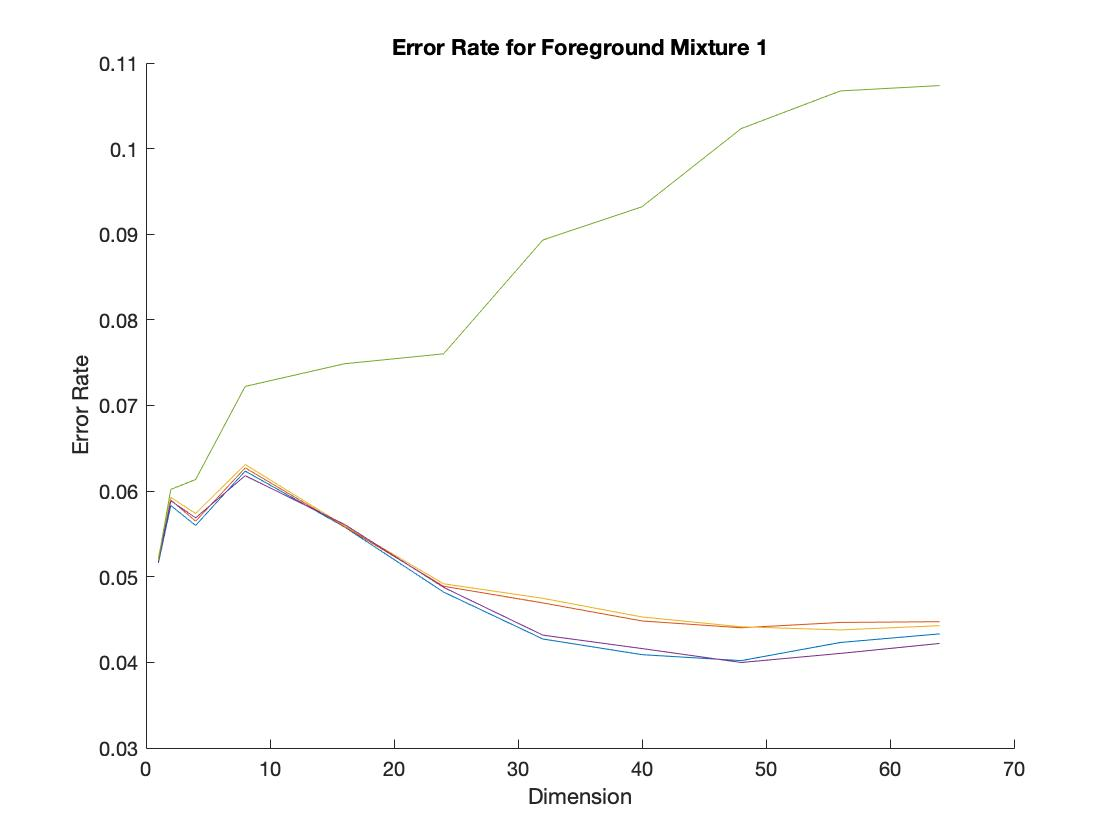
\includegraphics[scale=0.20]{part1_mix1.jpg}
		\caption{}
	\end{subfigure}
	% 
	\begin{subfigure}{0.5\textwidth}
		\centering 
		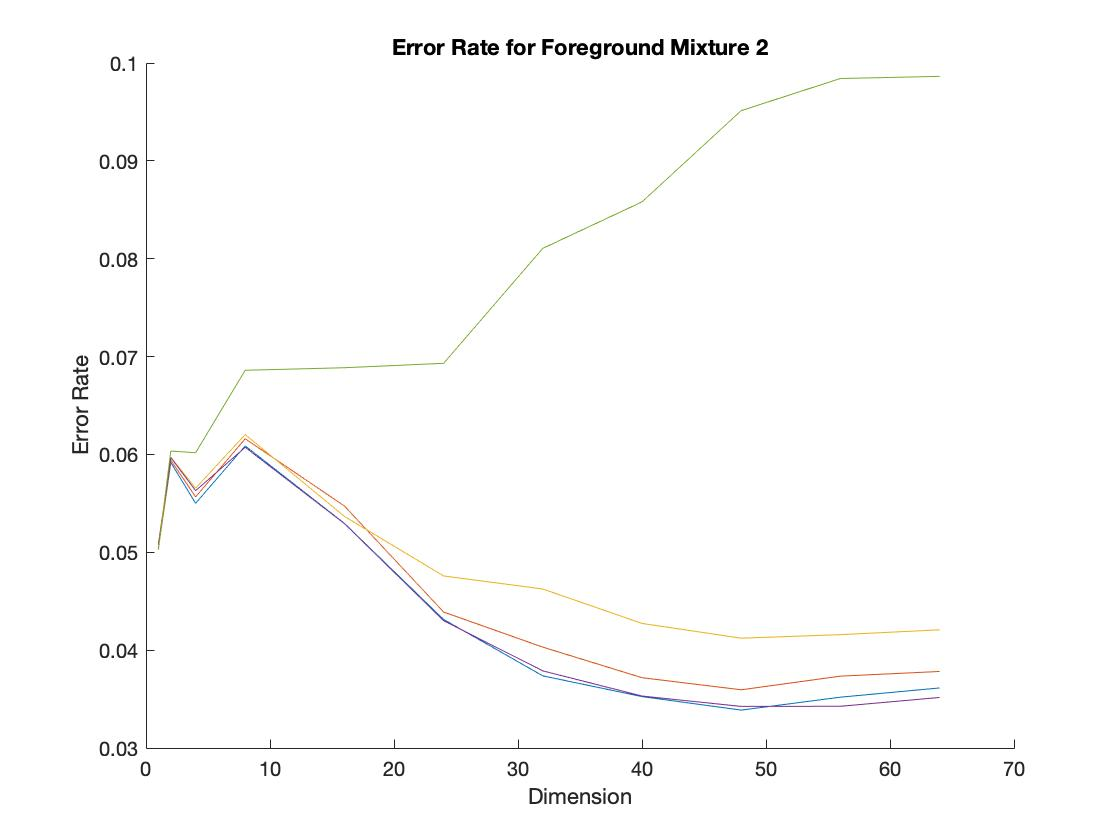
\includegraphics[scale=0.20]{part1_mix2.jpg}
		\caption{}
	\end{subfigure}
	% 
	\begin{subfigure}{0.5\textwidth}
		\centering 
		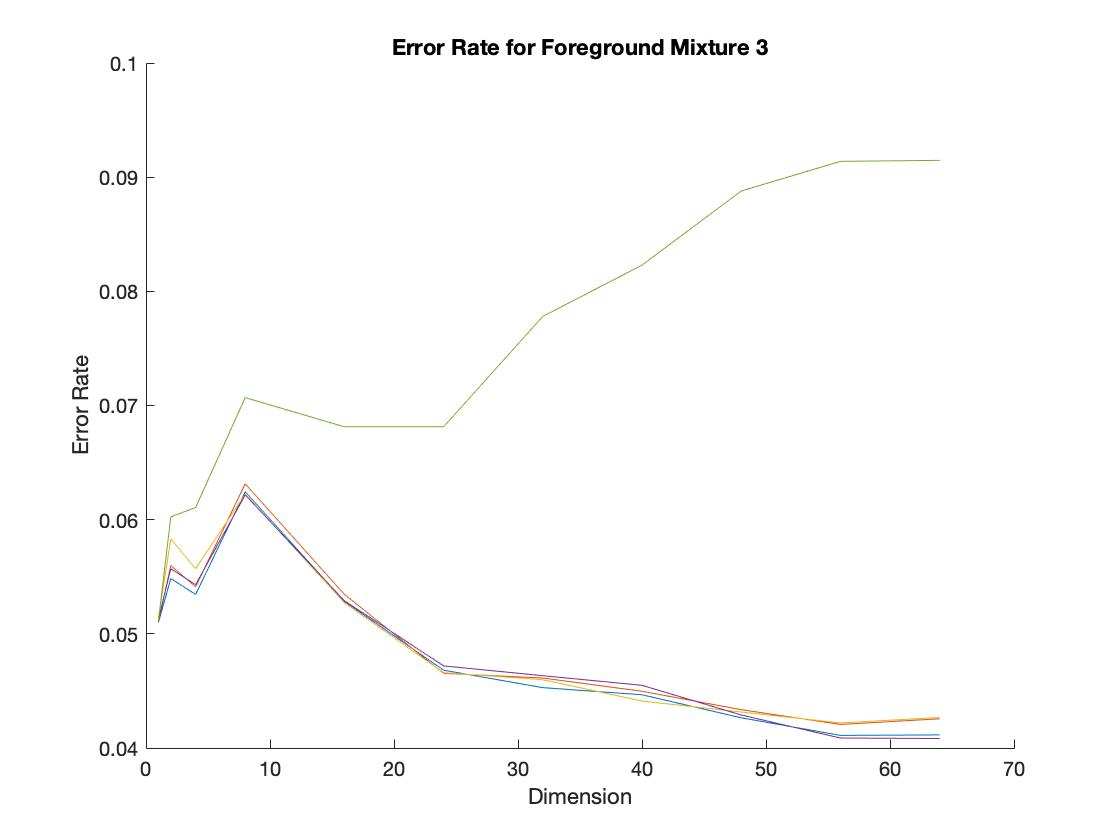
\includegraphics[scale=0.20]{part1_mix3.jpg}
		\caption{}
	\end{subfigure}
	% 
	\begin{subfigure}{0.5\textwidth}
		\centering 
		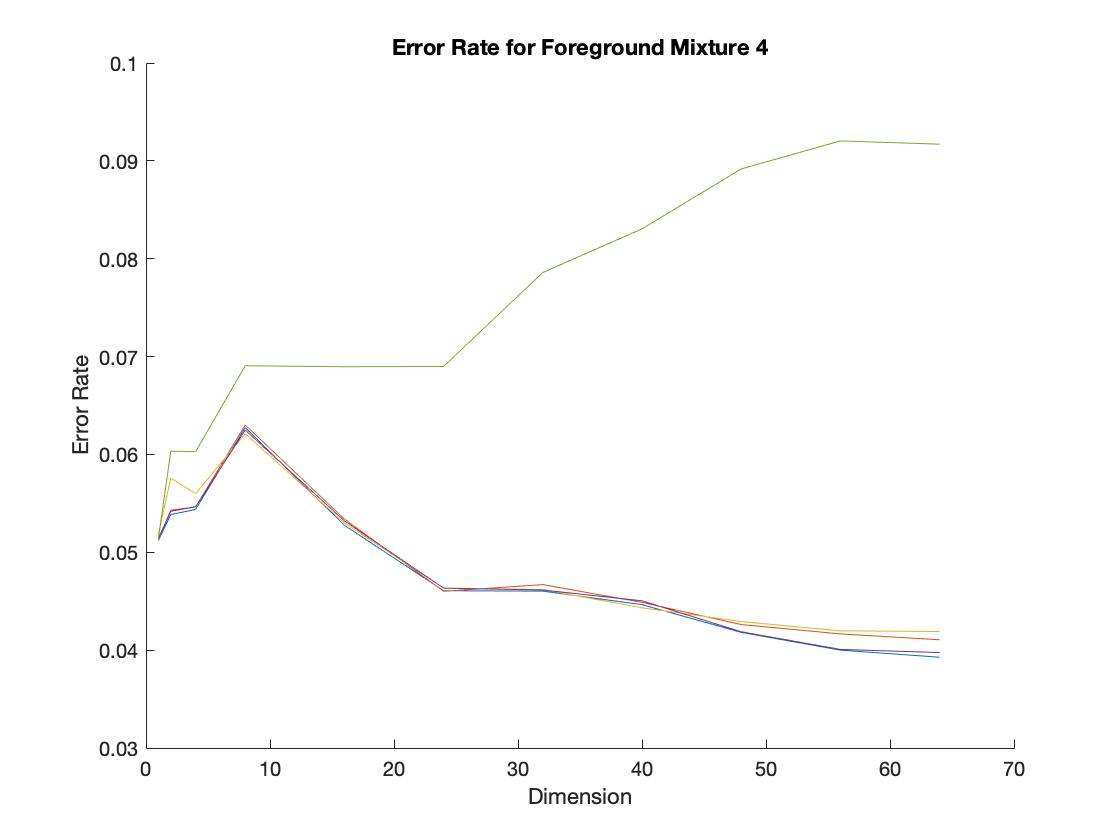
\includegraphics[scale=0.20]{part1_mix4.jpg}
		\caption{}
	\end{subfigure}
	% 
	\begin{subfigure}{0.5\textwidth}
		\centering 
		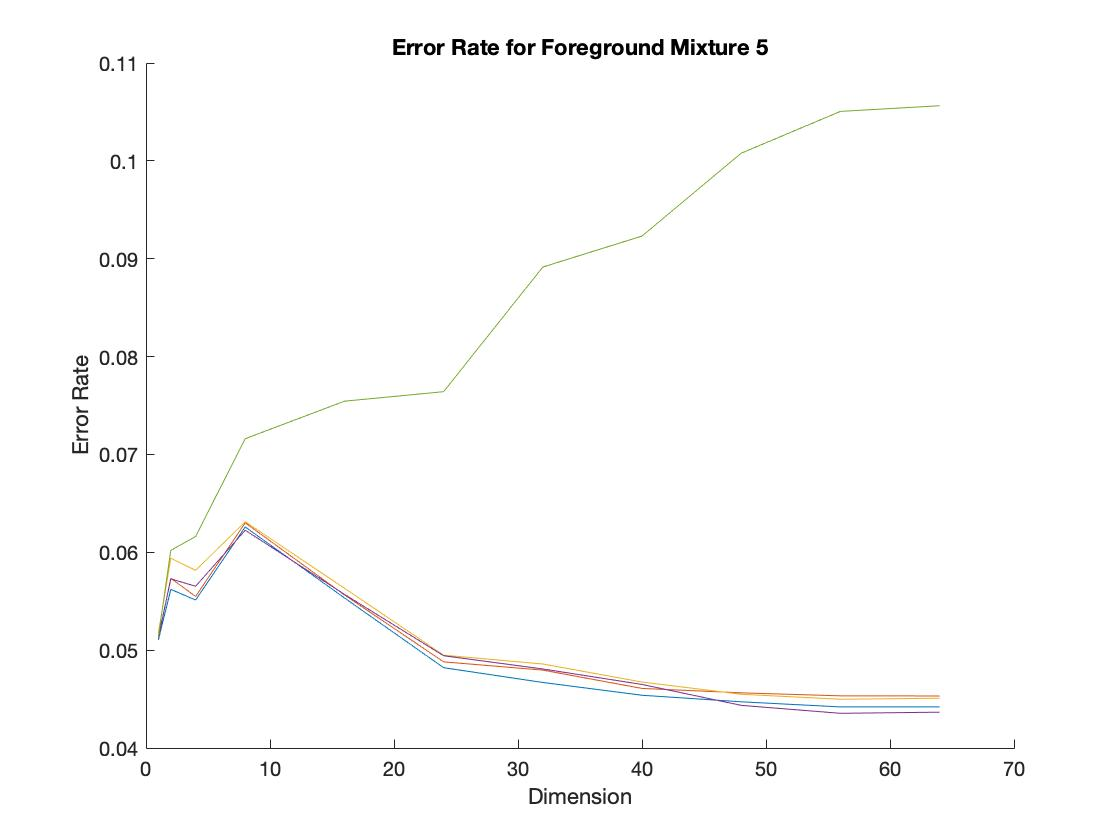
\includegraphics[scale=0.20]{part1_mix5.jpg}
		\caption{}
	\end{subfigure}
	\begin{subfigure}{0.5\textwidth}
		\centering 
		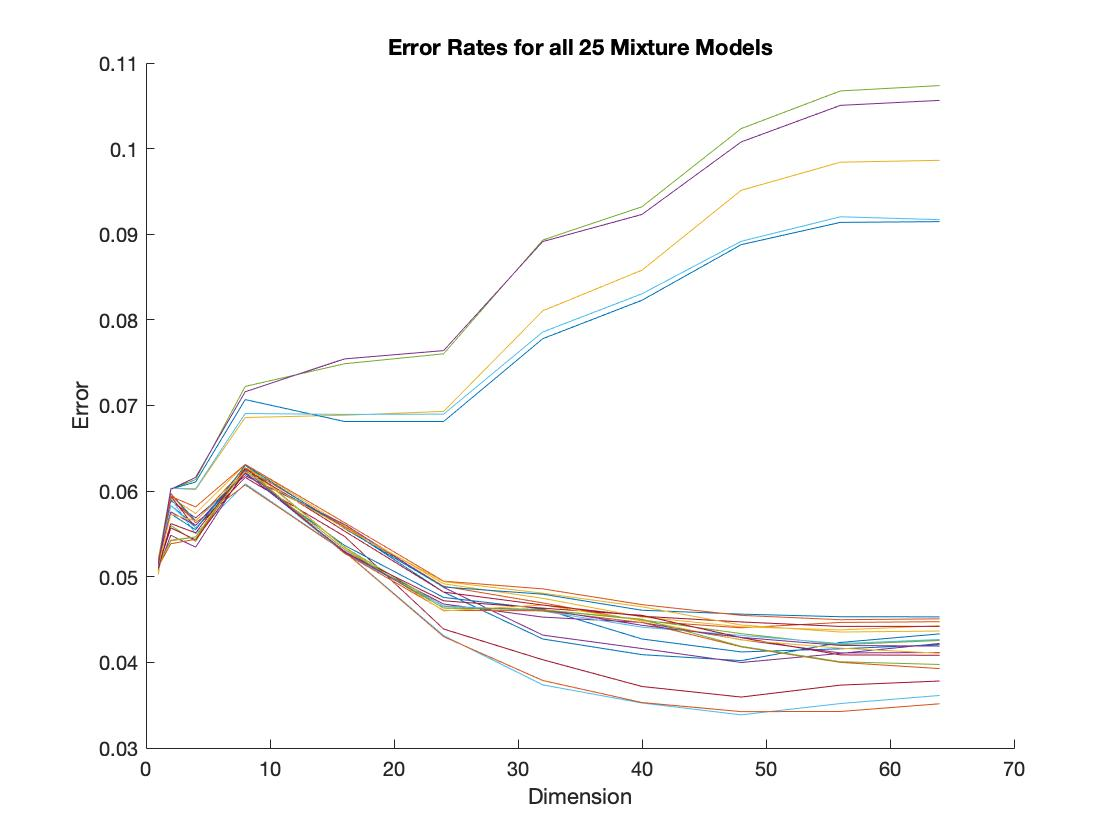
\includegraphics[scale=0.20]{part1_totalerror.jpg}
		\caption{}
	\end{subfigure}
	\caption{(a)-(e) Plots of the classification error as a function of the dimension, for the five background (BG) mixture models, with the corresponding FG mixture model. (f) Plot of the classification error as a function of the dimension for all $25$ mixture combinations.}
\end{figure}
\subsection{Analysis.}
One immediate observation is that the probability of error (POE), a way to measure the effectiveness of a classifier, is highly dependent on the intialization of the parameters. In figure 1, notice that there is one BG/FG mixture model pair that fares much worse than the others. The other pairs, compared to this one, have a lower POE and this difference becomes more apparent as the dimension size increases. As the dimension size increases we see that the initialization choice for the parameters can make the difference between an error of approximately $0.15$ or an error of approximately $0.045$. 

To explain the importance of a good initialization we rely on ideas from optimization theory. The EM algorithm is at its core, an \textit{iterative} algorithm that approximates the likelihood function in the presence of incomplete data. To be more specific, the EM algorithm can be used to approximate, or estimate, the parameters that define the likelihood function. In the case of the mixture of Gaussians (MOG) model, we estimate the likelihood function using $C$ weighted Gaussians with mean $\mu_c$ and $\sigma_c$, weighted by $\pi_c$. To estimate these parameters, the EM algorithm must maximize some function $f$ that depends on the parameters $\theta$, with respect to $\theta$. In general it is safe to assume that we will not always have access to information about $f$ itself (in particular we are interested in the number of maximums and minimums it attains). In the case where there are multiple maximums, the choice of our initial guess (which is required since EM is an iterative algorithm) becomes very important. Each maximum point has what is called a \textit{basin of attraction}. There is a theorem in the calculus of variations which states that all fixed points of some bounded functional $I$ that satisfies the Banach Fixed-Point theorem have a ball centered at the fixed point with radius $r$ such that initial guesses within that ball converge to the origin. To conclude, if a function $f$ has multiple maximums (or minimums) then our initial guess converges to the nearest maximum. Hence the bad FG/BG pair described above may have been the result of an initialization that led to another maximum point. 
\section{Part 2, $C \in \left\{ 1,2,4,8,16,32 \right\}$.}
\subsection{Results.}
\begin{figure}[H]
	\centering 
	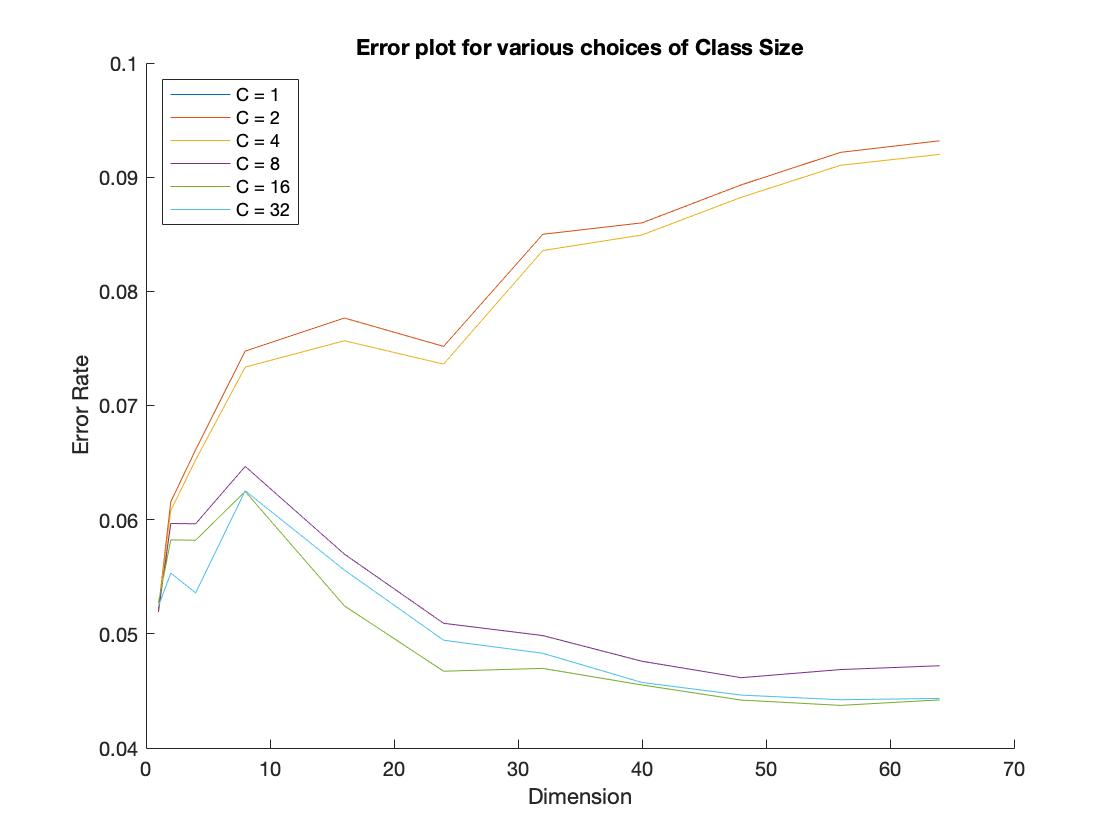
\includegraphics[scale=0.3]{part2_errorplot.jpg}
	\caption{Plot of the classification error as a function of the dimension, for different choices of $C$.}
\end{figure}
\subsection{Analysis.}
One immediate observation is the POE decreases as the number of classes and dimension size increases. In particular, when $C = 8,16,32$ we are able to achieve a POE less than $0.05$, as the dimension size increased. Under the MOG model, we essentially estimate the likelihood function by a weighted linear combination of Gaussians. By increasing the number of Gaussians used to estimate the likelihood function, we have a better change of fitting more complicated functions. This makes the classifier a bit more robust. However, we must be careful with the choice of $C$, since increasing the number of Gaussian classes \textit{also} increases the computation time, and we may have issues with overfitting/overestimating. 
\section{Conclusion.}
From the results above we cocnlude that the effectiveness of the classifier highly depends on the initialization of the parameters, the dimension of the classifier, and the nunmber of Gaussian classes used for estimating the likelihood function. The best POEs obtained from the EM method for the MOG model were much better than the POEs obtained in previous problem sets.
\section{MATLAB Code.} 
\lstinputlisting{em_main.m}
\lstinputlisting{em_calc.m}
\lstinputlisting{get_dct.m}
\lstinputlisting{bdr_predict.m}
\lstinputlisting{calc_prob.m}
\lstinputlisting{calc_error.m}

\end{document}